\documentclass[12pt,a4paper]{article}
\usepackage[UTF8]{ctex}
\usepackage{graphicx}
\usepackage{geometry}
\usepackage{ulem}
\usepackage{enumitem}
\usepackage{titlesec}
\usepackage{multicol}
\usepackage[export]{adjustbox}
\usepackage{amsmath}  % 推荐用于更好的数学排版
\usepackage[utf8]{inputenc}
\usepackage{CJKutf8}
\usepackage{fancyhdr}
\usepackage{lastpage}
\usepackage{ulem}
\usepackage{tabularx}
\usepackage{float}
\usepackage{siunitx}
\usepackage{multirow} 

% 页眉页脚设置
\pagestyle{fancy}
\fancyhf{} % 清除所有页眉页脚
% 设置页眉内容
%-==========1. 填写从第二页开始 每页第一行的信息==========-
\fancyhead[C]{\small
    \makebox[4.5em][c]{实验名称：} \uline{\makebox[17em][c]{集成运算放大器应用电路研究（II）}} 
    \makebox[2.5em][c]{姓名：} \uline{\makebox[4em][c]{}} 
    \makebox[2.5em][c]{学号：} \uline{\makebox[5em][c]{}}
}%--------------------------------------------------------
\fancyfoot[C]{\small 第 \thepage\ 页，共 \pageref{LastPage} 页}


% 取消页眉和页脚的下划线
\renewcommand{\headrulewidth}{0pt} % 页眉横线粗细设为0
\renewcommand{\footrulewidth}{0pt} % 页脚横线粗细设为0

% 调整页眉高度
\setlength{\headheight}{50pt}

% 设置plain样式（用于第一页）
\fancypagestyle{plain}{
    \fancyhf{} % 清除所有页眉页脚
    \renewcommand{\headrulewidth}{0pt} % 隐藏页眉横线
    \fancyfoot[C]{第 \thepage\ 页，共 \pageref{LastPage} 页} % 保留页脚
}
% 设置页面边距
\geometry{left=2.54cm,right=1.5cm,top=2.54cm,bottom=2.54cm}

% 设置正文字体大小为小四
\renewcommand{\normalsize}{\fontsize{12pt}{16pt}\selectfont}
% 设置章节格式
\titleformat{\section}{\fontsize{16pt}{22pt}\selectfont\bfseries}{\thesection}{1em}{} % 一级标题：三号
\titleformat{\subsection}{\fontsize{15pt}{20pt}\selectfont\bfseries}{\thesubsection}{1em}{} % 二级标题：小三

\begin{document}
\thispagestyle{plain}%第一页使用 plain 样式，而不是默认的 fancy 样式，第一页不再显示页眉
% 标题部分 - 两栏布局
\begin{multicols}{2}
    % 左栏：图片和实验报告标题
    % 左栏：使用空行创建前三行
    \noindent
    ~\\ % 第一行
    ~\\ % 第二行
    ~\\ % 第三行
    \hphantom{占位}% 使用空占位符
    \raisebox{-0.5\baselineskip}% 图片向下移动半行
    {
\includegraphics[width=1.85in,height=0.58in]{ZJU.jpg}}
    \hspace{.5em}% 图片和标题之间的间距
    \raisebox{0pt}[\height][0pt]% 标题底部对齐
    {\textbf{\fontsize{26pt}{30pt}\selectfont 实验报告}}
    
    \columnbreak % 换到右栏
    
    % 右栏：个人信息
    % 右栏：个人信息 - 靠右对齐 
%-==========2. 填写个人信息==========-
    \begin{flushright}
        \small
        \makebox[3em][l]{专业：} \uline{\makebox[9em][c]{法语-电子科学与技术}} \\
        \makebox[3em][l]{姓名：} \uline{\makebox[9em][c]{}} \\
        \makebox[3em][l]{学号：} \uline{\makebox[9em][c]{}} \\
        \makebox[3em][l]{日期：} \uline{\makebox[9em][c]{2025年12月23日}} \\
        \makebox[3em][l]{地点：} \uline{\makebox[9em][c]{紫金港东四216}} \\
    \end{flushright}   
\end{multicols}
% 课程名称等信息（单栏）
%-==========3. 填写课程信息==========-

{\small
\noindent
课程名称： \uline{电子电路设计实验I} \hfill 指导老师： \uline{施红军、叶险峰、邓靖靖} \hfill 成绩： \uline{\hspace{3cm}} \\
实验名称：\uline{集成运算放大器应用电路研究（II）}\hfill 实验类型：\uline{设计实验}\hfill 同组学生姓名：\uline{}
}
%-==========4. 正文开始==========-
\section*{一、实验目的}
1、学习和研究由集成运放构成的积分器、比较器、波形发生器等应用电路的组成与原理，掌握其设计方法。

2、观察积分运算电路在实际应用时存在的积分漂移、积分误差等现象，了解解决方法。


\section*{二、实验任务与要求}

\textbf{1、反相积分器设计研究}

（1）设计反相积分电路，方波$\Rightarrow$ 三角波。其中方波幅度2.2V、频率500Hz；三角波，幅度2V左右。

（2）安装该电路，输入方波，用示波器双踪显示输入、输出波形，测量并记录波形，标示出各实测参数。


\textbf{2、迟滞比较器设计研究}

（1）设计一迟滞比较器，使\[V_{TH}\approx \frac{V_Z+V_D}{2}\]

允许使用电阻值在20kΩ至400kΩ之间。

（2）安装电路，输入500Hz三角波（幅度合理自定），研究输入、输出信号的幅度、相位关系。


\textbf{3、方波-三角波发生器研究}

断开迟滞比较器信号输入，搭建方波-三角波发生电路，调节电位器$R_{w4}$，可产生不同频率方波、三角波。观察电压$V'_{42o}$与输出信号频率的关系，测量并记录可调频率范围。


\section*{三、实验原理}


\subsection*{3.1 反相积分器}
\begin{figure}[H]
    \centering
    
\includegraphics[width=0.3\textwidth]{1.png}
    \caption{反相积分器电路}
    \label{fig1}
    \end{figure}
输出电压
\[
V_0(t) = -\frac{1}{C} \int_{0}^{t} \frac{V_i(t)}{R_1} \, dt= -\frac{1}{R_1 C} \int_{0}^{t} V_i(t) \, dt
\]

当输入信号为一阶跃信号时，

\[
V_i(t) =
\begin{cases}
0, & t < 0 \\
E, & t \geq 0
\end{cases},
V_0(t) = -\frac{E}{R_1 C}t
\]


积分器可以将方波转化为三角波，输入输出电压峰值之间的关系为
\[2B = \frac{A}{R_1 C}\cdot \frac{T}{2} \Rightarrow R_1 = \frac{AT}{4BC}\]
\begin{figure}[H]
    \centering
    
\includegraphics[width=0.3\textwidth]{5.png}
    \caption{将方波转化为三角波}
    \label{fig5}
    \end{figure}

输入信号的直流分量、输入失调电压等会形成积分漂移。

实际使用时，常在积分电容的两端并联一个电阻 \( R_f \)，形成直流负反馈，用以限制电路的直流电压增益。  
\( R_f \) 的接入将对积分电容产生分流作用，从而导致积分误差。
\begin{figure}[H]
    \centering
    
\includegraphics[width=0.3\textwidth]{2.png}
    \caption{修正积分漂移}
    \label{fig2}
    \end{figure}
为了减小积分误差，一般要求 
\[ R_f > \frac{1}{j\omega C} \text{，或 } f > \frac{1}{2\pi R_f C} \]此时 \( R_f \) 可认为开路（理想积分器）。  
由 \[ R_f > \frac{1}{2\pi fC}, 2B = \frac{A}{R_1 C} \cdot \frac{T}{2} \Rightarrow R_f > \frac{2B}{\pi A} R_1 \]通常取 \[ R_f > 10R_1 \]

\subsection*{3.2 迟滞比较器}

\begin{figure}[H]
    \centering
    
\includegraphics[width=0.3\textwidth]{4.png}
    \caption{迟滞比较器电路}
    \label{fig4}
    \end{figure}


\begin{enumerate}
    \item[(1)] 当 \( V_6 = V_{OH} \) 时,
          \[
          V'_+ = \frac{R_{43}}{R_{43}+R_{44}}(V_{Z2} + V_{D1}) + \frac{R_{44}}{R_{43}+R_{44}}V_{42i}
          \]
    
    \item[(2)] 当 \( V_6 = V_{OL} \) 时,
          \[
          V''_+ = -\frac{R_{43}}{R_{43}+R_{44}}(V_{Z1} + V_{D2}) + \frac{R_{44}}{R_{43}+R_{44}}V_{42i}
          \]
    
    \item[(3)] 当 \( V_6 = V_{OH} \) 时,
          \[
          V'_+ = \frac{R_{43}}{R_{43}+R_{44}}(V_{Z} + V_D) + \frac{R_{44}}{R_{43}+R_{44}}V_{42i}
          \]
    
    \begin{itemize}
        \item 要使输出稳定为 \( V_{OH} \), \( V'_+ > 0 \), \( V_{42i} > -\frac{R_{43}}{R_{44}}(V_{Z} + V_D) = -V_{TH} \)
        \item 要使输出翻转为 \( V_{OL} \), \( V'_+ < 0 \), \( V_{42i} < -V_{TH} \)
    \end{itemize}
    
    \item[(4)] 当 \( V_6 = V_{OL} \) 时,
          \[
          V''_+ = -\frac{R_{43}}{R_{43}+R_{44}}(V_{Z} + V_D) + \frac{R_{44}}{R_{43}+R_{44}}V_{42i}
          \]
    
    \begin{itemize}
        \item 要使输出稳定为 \( V_{OL} \), \( V''_+ < 0 \), \( V_{42i} < V_{TH} \)
        \item 要使输出翻转为 \( V_{OH} \), \( V''_+ > 0 \), \( V_{42i} > V_{TH} \)
    \end{itemize}
\end{enumerate}

输出为\[V_{Th}=\frac{R_{43}}{R_{44}}(V_Z+V_D)\]

\begin{figure}[H]
    \centering
    
\includegraphics[width=0.3\textwidth]{6.png}
    \caption{理论传输特性曲线}
    \label{fig6}
    \end{figure}

\begin{figure}[H]
    \centering
    
\includegraphics[width=0.3\textwidth]{7.png}
    \caption{输入输出波形}
    \label{fig7}
\end{figure}



\section*{四、实验方案设计与参数计算}

\subsection*{4.1 反相积分器设计}

反相积分器采用如图\ref{fig1}所示的电路，只需要确定参数即可。

设计要求方波幅度2.2V、频率500Hz；三角波，幅度2V左右，其中电容\(C=0.022\mu\text{F} \)由此
\[A=2.2\text{V}, f=500\text{Hz}, B=2\text{V}, T=0.002\text{s}\]
则
\[2B = \frac{A}{R_1 C}\cdot \frac{T}{2} \Rightarrow R_1 = \frac{AT}{4BC}=25\text{k}\Omega\]

取标称值\(R_1=24\text{k}\Omega\)。

反馈电阻取 \[ R_f > 10R_1 \Rightarrow R_f = 270\text{k}\Omega \]


\subsection*{4.2 迟滞比较器设计}

迟滞比较器采用如图\ref{fig4}所示的电路，只需要确定参数即可。 

实验要求\[V_{TH}\approx \frac{V_Z+V_D}{2}\]则\[\frac{R_{43}}{R_{44}}=\frac{1}{2}\]

且允许使用电阻值在20kΩ至400kΩ之间，则取
\[R_{43}=100\text{k}\Omega, R_{44}=200\text{k}\Omega\]

\subsection*{4.3 方波-三角波发生器}

方波-三角波发生器采用如下所示的电路。

\begin{figure}[H]
    \centering
    
\includegraphics[width=0.6\textwidth]{8.png}
    \caption{发生器实验电路}
    \label{fig8}
    \end{figure}

\begin{figure}[H]
\centering
    
\includegraphics[width=0.6\textwidth]{9.png}
    \caption{发生器实验波形}
    \label{fig9}
        \end{figure}



\section*{五、实验仪器设备}

直流稳压电源、信号源、示波器。

\section*{六、实验步骤、调试过程、实验数据记录}

\subsection*{6.1 反相积分器}
安装电路，输入幅度2.2V、频率500Hz的方波，用示波器双踪显示输入、输出波形。
\begin{figure}[H]
    \centering
    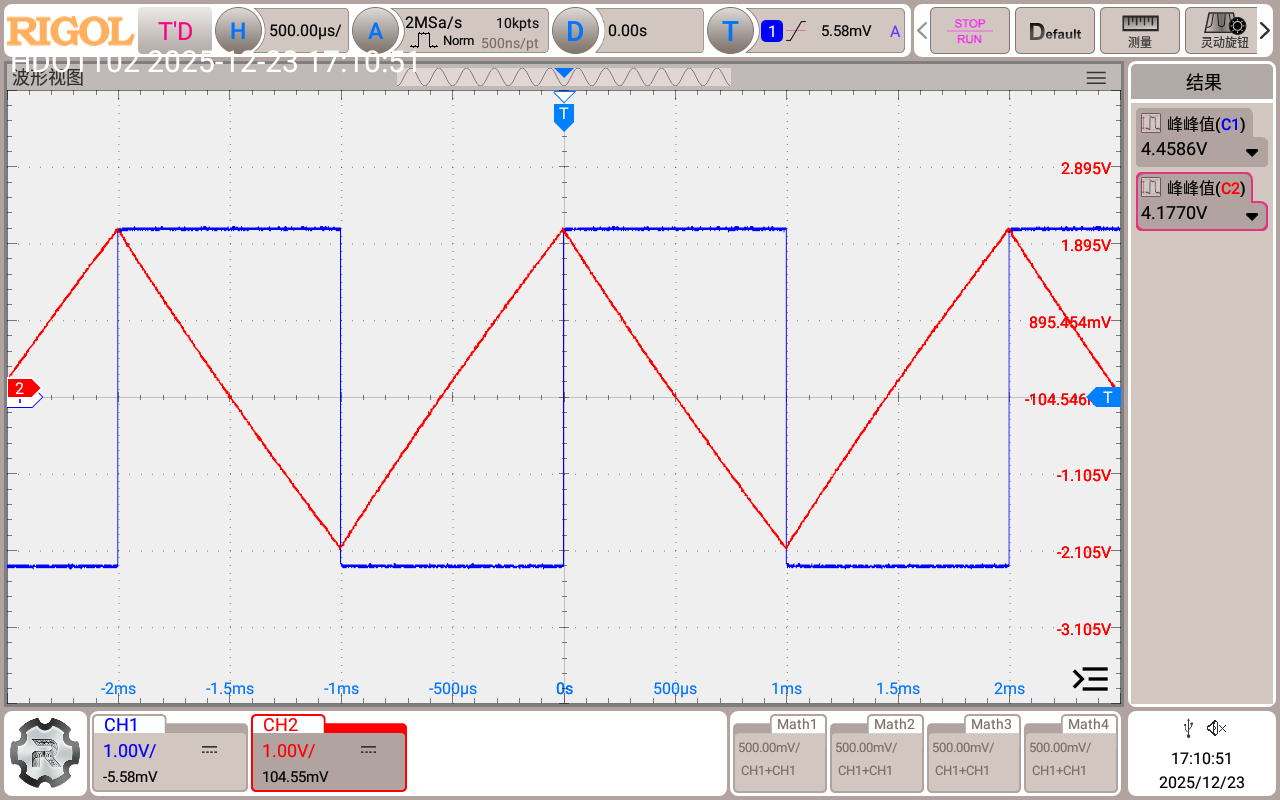
\includegraphics[width=0.8\textwidth]{30.png}
    \caption{反相积分器输入输出波形}
    \label{fig30}
    \end{figure}
可以看出输入方波峰峰值4.4586V，输出三角波峰峰值4.1770V。符合要求。插入反馈电阻\(R_f\)时，测得直流偏移量为209.06mV；拔下反馈电阻\(R_f\)时，测得直流偏移量为1.39V。
\subsection*{6.2 迟滞比较器}
安装电路，输入输入幅度4V（输入幅度应大于门限电压$V_{TH}$）、频率500Hz的三角波，用示波器双踪显示输入、输出波形。

可以看出输入三角波峰峰值7.8549V，输出方波峰峰值14.046V。利用光标测得门限电压$V_{TH}$约为3.585V。

\begin{figure}[H]
    \centering
    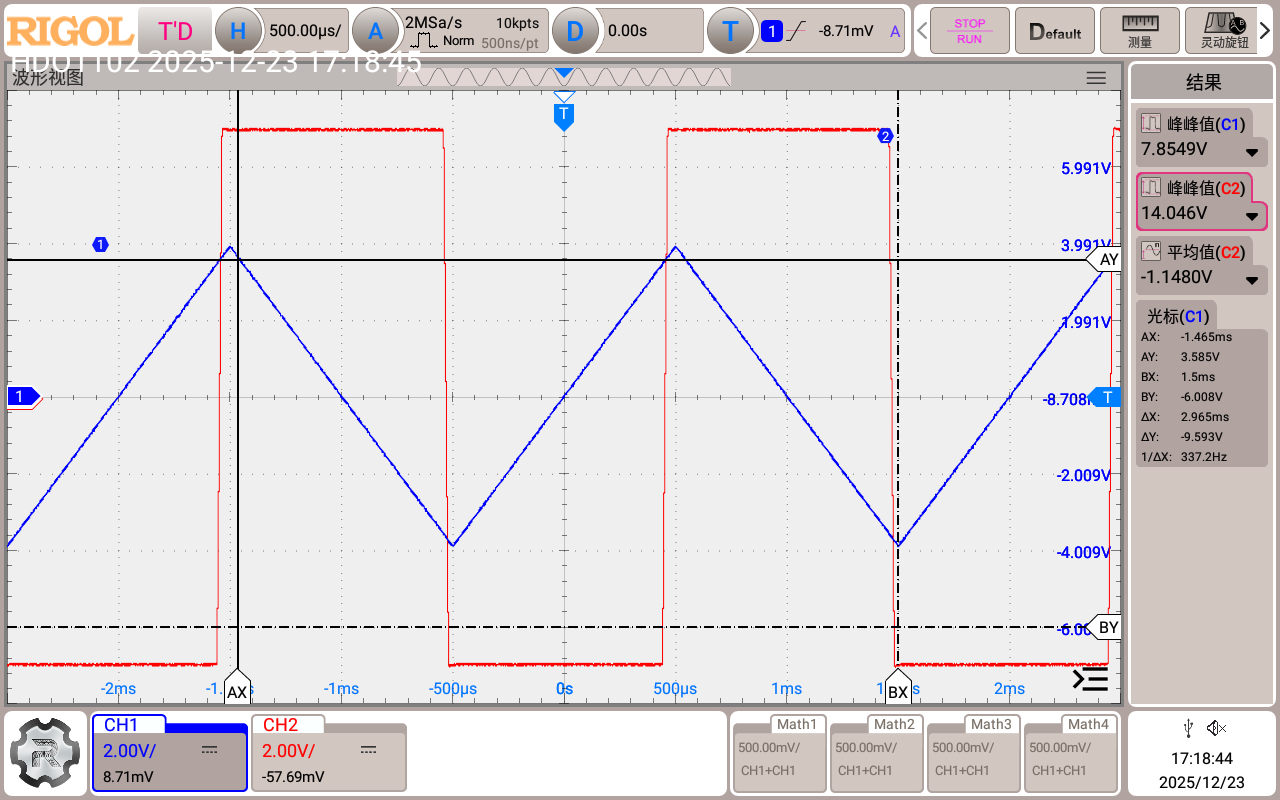
\includegraphics[width=0.8\textwidth]{35.png}
    \caption{迟滞比较器输入、输出波形}
    \label{fig35}
    \end{figure}
    


\subsection*{6.3 方波-三角波发生器}

断开迟滞比较器信号输入，搭建方波-三角波发生电路，调节电位器$R_{w4}$，可产生不同频率方波、三角波。

调节电位器$R_{w4}$，观察到输出信号频率越大，电压$V'_{42o}$越大。

\begin{figure}[H]
    \centering
    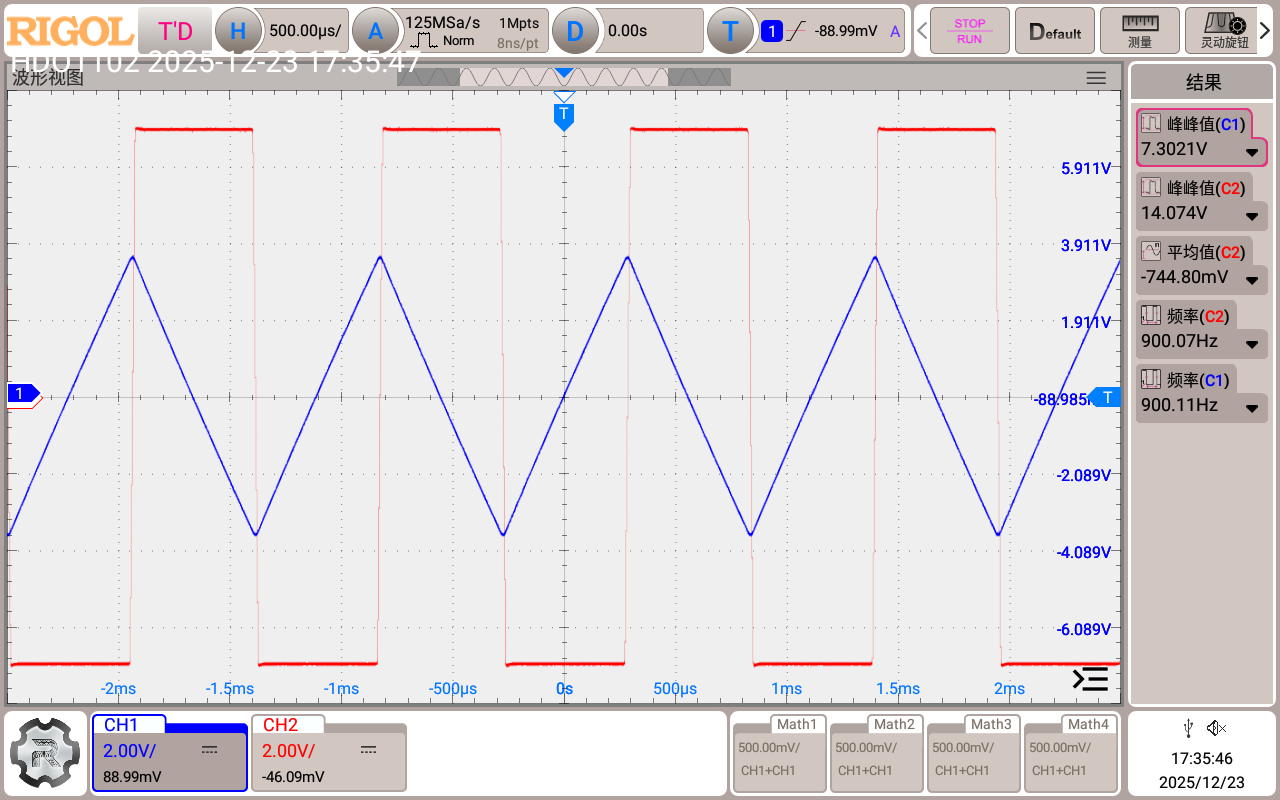
\includegraphics[width=0.8\textwidth]{39.png}
    \caption{方波-三角波发生器波形}
    \label{fig39}
    \end{figure}

频率调整上限约为900Hz，下限很小，但频率低时三角波会失真。

\begin{figure}[H]
    \centering
    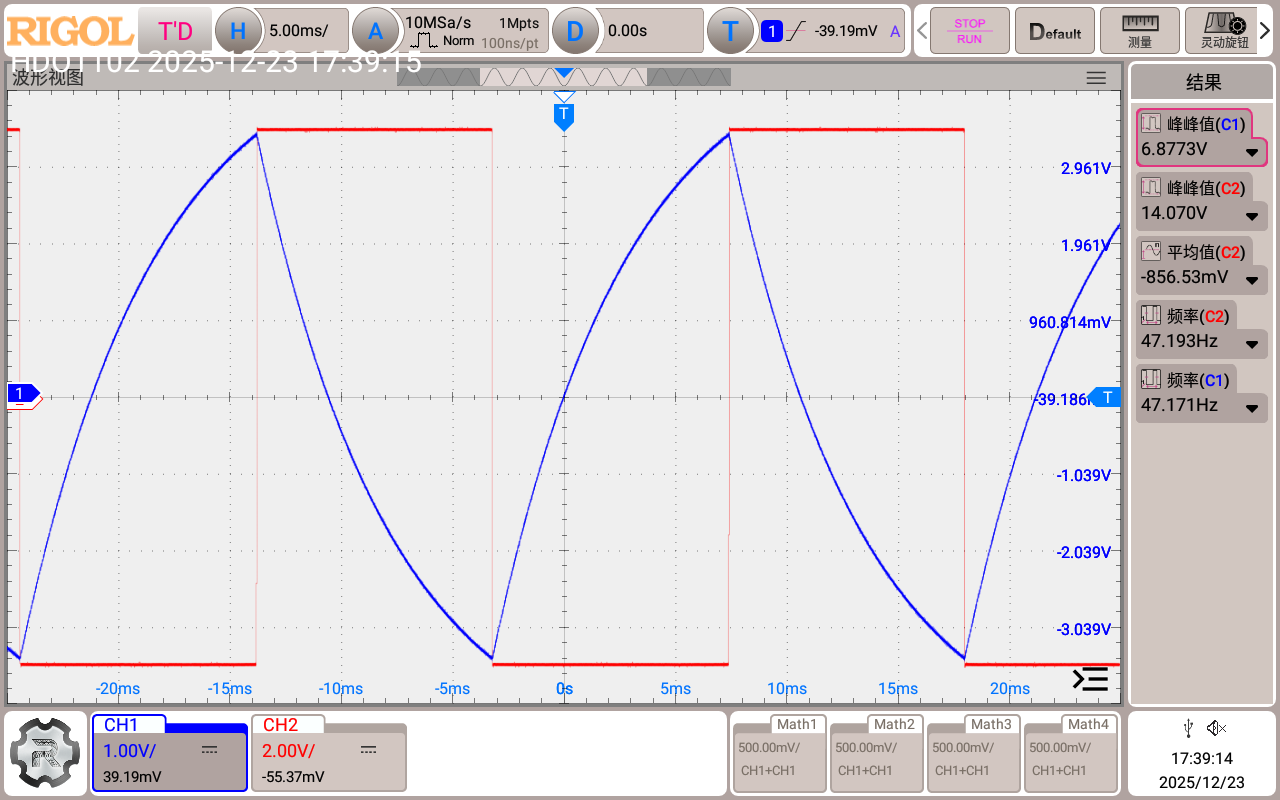
\includegraphics[width=0.8\textwidth]{40.png}
    \caption{频率低时三角波的失真}
    \label{fig40}
    \end{figure}
    





\section*{七、心得与体会}

通过本次实验，我对积分、比较与波形发生三类电路的原理与实现有了更深入的认识，积累了从设计到调试的完整工程经验。

在反相积分器实验中，我直观观察到积分漂移现象。未接入反馈电阻时，输出直流偏移达1.39V，接入270kΩ反馈电阻后偏移降至209.06mV。这使我深刻理解到，理论设计中抑制误差的措施在实际电路中的必要性。设计时需在理想模型与工程实现间取得平衡。

迟滞比较器的调试让我认识到门限设置的重要性。输入信号幅度必须大于设计阈值，电路才能正常翻转。实测阈值电压为3.585V，与理论计算基本吻合。通过双踪观察输入三角波与输出方波，我清晰理解了回差电压对波形转换的关键作用。

在方波-三角波发生器实验中，我通过调节电位器实现了频率可调，但也发现低频时三角波出现失真。这反映出积分时间常数与波形质量的制约关系，提示我们在实际系统设计中需综合考虑频率范围与波形完整性。

总体而言，本次实验不仅巩固了课堂所学，更锻炼了我依据实测现象分析问题、优化参数的能力。我认识到，一个成功的电路设计既需要严谨的理论计算，也离不开细致的调试与验证。


\end{document}